\documentclass[USenglish]{article}

\usepackage{ifikompendiumforside}
\usepackage{graphicx}

\title{Improving the performance of Web Services in Disconnected, Intermittent and Limited Environments}
\author{Joakim Johanson Lindquister}

\begin{document}
\ififorside{}

\begin{abstract}
    My abstract
\end{abstract}

\part{Introduction}
\section{Motivation}
\section{Problem Statement}
Most of the Web Service solutions used today are aimed for civilian use and does not necessarily perform well in military environments. In contrast to civilian networks where bandwidth are abundant, mobile tactical networks may suffer from high error rates and low bandwidth. In my master thesis I will investigate how communication between two clients running at two separate machines can be improved by using a proxy deployed at each machine. The Web Services will communicate with his counter part over HTTP as regular, with all traffic going umerkelig through the proxy. The Web Service itself does not need to pay attention to the bad connectivity, the proxy will choose the appropriate protocol and configuration.
\section{Research Method}
\section{Contribution}
\section{Outline}

\part{Background}

\part{Design and Implementation}
\section{Proxy}
\begin{figure}[h]
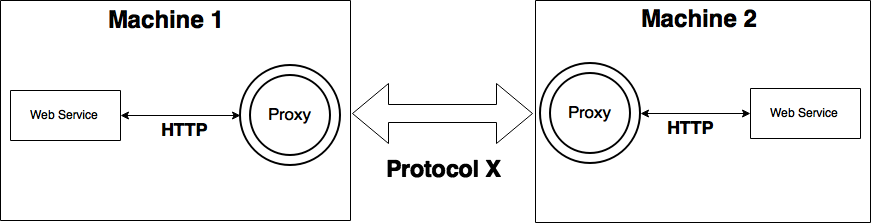
\includegraphics[scale=0.4]{images/architecture.png}
\caption{Architectural overview of proposed design}
\end{figure}


\part{Testing and Evaluation}

\end{document}
